% !TeX root = ../main.tex

\section{Results}\label{sec:evaluation}


\subsection{Prevalence Study (RQ1)}

\begin{figure*}[!t]
    \centering
    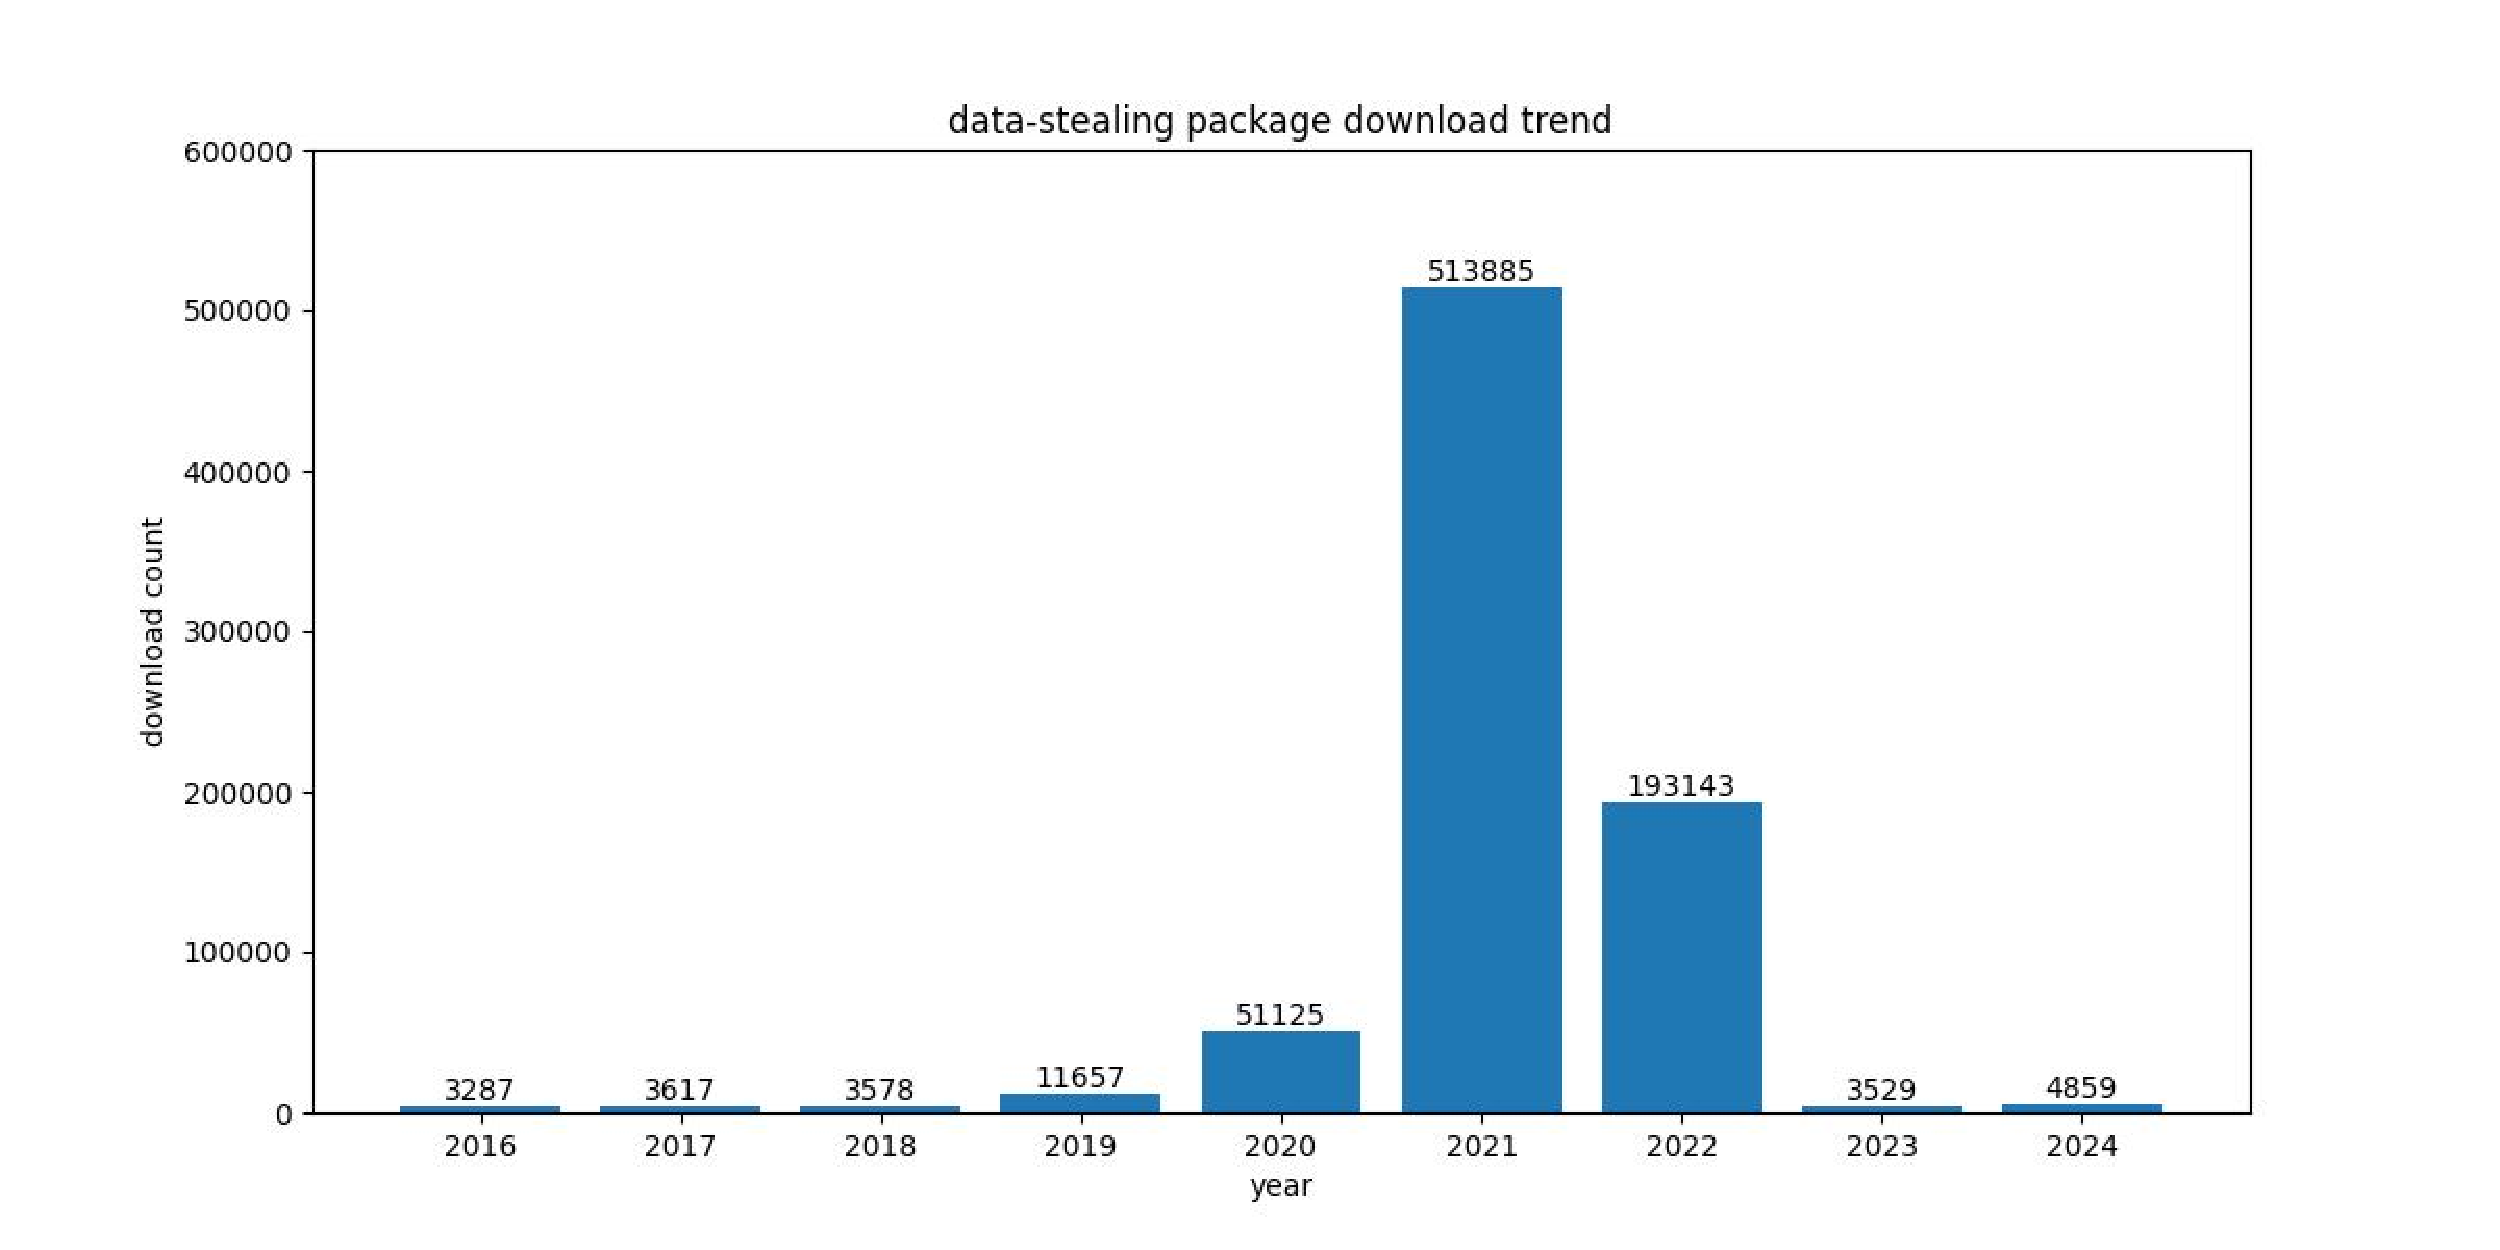
\includegraphics[width=1.0\textwidth]{fig/download_count.pdf}
    \vspace{-10pt}
    \caption{Download Trends of Data-Stealing Packages (2017–2024)}
    \label{fig:mitigationoverview}
\end{figure*}

By collecting and counting the download data of the classified data-stealing packages, we generated a trend chart covering the period from 2017 to 2024, as depicted in Fig.1.
The statistical chart shows that the package downloads gradually increased from 2017 to 2022, with a larger growth rate in 2021 and 2022, reaching a peak in 2021,then declined in 2023 and 2024.

We found that 2021 was a period of outbreak of malicious packages.At the same time, the download volume in 2020 cannot be ignored.In 2021, software supply chain attacks became a major trend in cybercrime, and attackers began to exploit open source software repositories (such as PyPI, npm, and RubyGems) on a large scale.
Furthermore,since PyPI prioritizes installing the latest versions of libraries by default, attackers can upload malicious updates on PyPI and trick developers into downloading them.
The 2020-2021 SolarWinds hack was one of the most serious supply chain attacks in recent years.The success of hackers using supply chain vulnerabilities to break into the U.S. government and companies had brought supply chain attacks into the public eye, and as a result, the hacker community had begun to use PyPI more frequently to spread malware.
Additionally, on June 23,2022, the OSCS,open source security community monitoring found that the PyPI official repository was uploaded by the attacker mega707 with more than 150 malicious phishing packages such as `agoric-sdk` `datashare` `datadog-agent`.
%https://www.oscs1024.com/hd/MPS-2022-20159
%https://www.solarwinds.com/sa-overview/securityadvisory

The decrease in downloads in 2023 and 2024 is speculated to be caused by restrictions imposed by the PyPI.
On May 25, 2023, PyPI announced that every account that maintains any project or organization on PyPI will be required to enable Two-factor authentication (2FA) on their account by the end of 2023.And On January 1, 2024, PyPI requires 2FA for all users.
%https://blog.pypi.org/posts/2023-05-25-securing-pypi-with-2fa/
%https://blog.pypi.org/posts/2024-01-01-2fa-enforced/
Prior to this measure, if someone used a simple or reused password, an attacker could take control of the maintainer's account and begin acting as that user, while installing and executing software on unsuspecting users' computers.
Enabling 2FA makes it almost impossible for an attacker to directly control the PyPI maintainer's account even if they steal the password, significantly reducing the risk of legitimate accounts being hijacked to upload malicious packages. This is critical to the security of the PyPI ecosystem and helps protect developers and users from malware.

\subsection{Pattern Study (RQ2)}
In this section, we present a detailed analysis of the attack patterns employed by data-stealing malicious packages. By meticulously examining the source code of these packages, we summarize and classify the attack patterns and processes of the packages, and count the proportion of each mode, as shown in Table 2.
In this section, we mainly study the attack patterns. Therefore, in Table 2,the stolen information we recorded is the main stolen information, and the attached stolen information is not recorded in detail.

\begin{longtable}{>{\hspace{0pt}}m{0.065\linewidth}|>{\centering\hspace{0pt}}m{0.769\linewidth}|>{\centering\arraybackslash\hspace{0pt}}m{0.102\linewidth}} 
    \hline
    \multicolumn{1}{>{\centering\hspace{0pt}}m{0.065\linewidth}|}{Pattern} & Description                                                                                                     & Percentage  \endfirsthead 
    \hline
    1                                                                     & decrypt authentication information->steal personal, system info->(encrypt info)->packaging info->transmit              & 7.2\%       \\ 
    \hline
    2                                                                     & decrypt authentication information->steal personal, system info->(encrypt info)->packaging info->transmit->extra attack              & 3.6\%       \\ 
    \hline
    3                                                                     & steal system info->packaging info->(encrypt info)->transmit                                                         & 72.3\%      \\ 
    \hline
    4                                                                     & steal system info->transmit->remote download->execute downloaded files                                              & 10.8\%      \\ 
    \hline
    5                                                                     & steal system info->transmit->extra attack                                                                          & 1.2\%       \\ 
    \hline
    6                                                                     & steal financial info->packaging info->transmit                                                                     & 1.2\%       \\ 
    \hline
    7                                                                     & steal personal,financial info->packaging info->transmit->extra attack                                               & 1.2\%       \\ 
    \hline
    8                                                                     & steal system,software info(configuration file)->transmit                                                          & 1.2\%       \\ 
    \hline
    9                                                                     & steal authentification info->transmit                                                                             & 1.2\%       \\
    \hline
    \caption{Attack Pattern Classification and Statistics}
    \end{longtable}

\par The packages represented by pattern 1 are mainly based on website, browser and software.They mainly steal user information, payment information, browsing history and automatic filling information from these platforms.
To steal the information stored on the platform, the package needs to obtain the master key or tokens to control the account.
\par The master key is an AES encryption key used by chromium browsers (such as chrome, edge and brake) to protect locally stored passwords, cookies and credit card information.This key is stored in the \textit{local state} file and encrypted through the windows DPAPI.
To obtain the master key, the package will first find the local state file, which is usually stored in the path \textit{appdata/local/google/chrome/user data/local state}.
Then the packages read the encrypted\_key field, decrypt it using windows DPAPI, and then decrypt the stored data such as passwords and cookies using the decrypted master key.The specific code is shown in Listing 1.
\par The browser usually provides the "save password" function. When a user logs in to a website \textit{(e.g. email, social media)}, the browser will prompt the user whether to save the password. If the user chooses to save, the browser will encrypt the website address, user name and password and store them locally. 
Cookies are small data files stored in the user's browser by the website, which are used to maintain the user's login status and other preferences. When a user logs in to a website, the server will generate a session cookie and send it to the user's browser. The browser will save this cookie and automatically send it to the server in subsequent requests to verify the user's identity.
After the script steals the master key, it can decrypt and obtain these passwords and cookies,then log in directly to the user's online account,or use cookies for session hijacking and impersonate users to access online services.Finally, steal users' personal information stored on the website.
%%%%%%%%%%%%%%%%%%%%%%%%%%%%%%%%%%%%%%%%%%%%%%%%% 展示代码片段
\begin{lstlisting}[caption={Steal Master key}, label={code:masterkey}]
def get_master_key(path: str):
    with open(path + "\\Local State", "r", encoding="utf-8") as f:
        c = f.read()
    local_state = json.loads(c)
    master_key = base64.b64decode(local_state["os_crypt"]["encrypted_key"])
    master_key = master_key[5:]
    master_key = CryptUnprotectData(master_key, None, None, None, 0)[1]
    return master_key
    \end{lstlisting}
%%%%%%%%%%%%%%%%%%%%%%%%%%%%%%%%%%%%%%%%%%%%%%%%
\par A token is a short-term valid credential used to bypass traditional password authentication and directly log in to an account.After stealing the token, the attacker can access the account for a short time.
Tokens are usually stored in the \textit{/local storage/leveldb}.The data-stealing packages always define a list called \' path \', add the paths where various browsers and softwares store \textit{leveldb} files to the list, and then traverse these paths to find matching tokens.
The \' Path \' usually covers many mainstream browsers and software, including opera, Microsoft edge, chrome, discord canary, discord PTB, etc., to improve the success rate of stealing.
If a browser or software is installed on the host, they will get its tokens smoothly.The specific code is shown in Listing 2.
%%%%%%%%%%%%%%%%%%%%%%%%%%%%%%%%%%%%%%%%%%%%%%%%
\begin{lstlisting}[caption={Steal Tokens}, label={code:masterkey}]
def tokens(ctx):
    paths = [
        os.path.join(os.getenv("APPDATA"), ".discord"/".discordcanary"/".discordptb", "Local Storage", "leveldb"),
        os.path.join(os.getenv("LOCALAPPDATA"), "Google"/"Microsoft"/"BraveSoftware", "Chrome"/"Edge"/"Brave-Browser",, "User Data", "Default", "Local Storage", "leveldb"),
        os.path.join(os.getenv("APPDATA"), "Opera Software", "Opera Stable"/"Opera GX Stable", "Local Storage", "leveldb"),]
    tokens = []
    for path in paths:
        for file in os.listdir(path):
            for line in [x.strip() for x in open(os.path.join(path, file), errors="ignore").readlines() if x.strip()]:
                for regex in [r"[\w-]{24}\.[\w-]{6}\.[\w-]{38}", r"mfa\.[\w-]{84}"]:
                    for token in re.findall(regex, line):
                        account_name = get_account_name(token)
                        tokens.append((account_name, token))
        \end{lstlisting}
%%%%%%%%%%%%%%%%%%%%%%%%%%%%%%%%%%%%%%%%%%%%%%%可能需要缩减一下，过长了
\par After obtaining the token, some scripts will verify the validity of the token. Take discord as an example. If the incoming token is in the self.tokens list, continue processing. 
Then generate the request header through \textit{self.getheaders (token)}, and send a request to discord's API using \textit{requests.get} to verify the validity of the token. Check the response status code through complex bit operation. If the request is successful and the token is not in the self.tokens list, add the token to the list.
\par After obtaining a valid discord token, the script will request the account details through the Discord API. The script will also set the HTTP request header, and then send HTTP get requests to different API endpoints of Discord to return sensitive information such as user basic information, payment information, and friends list.

%%%%%%%%%%%%%%%%%%%%%%%%%%%%%%%%%%%%%%%%%%%%%%%%
\begin{lstlisting}[caption={Request Header Example}, label={code:masterkey}]
    headers=
    {'Authorization':token,
        'Content-Type':'application/json',
        'User-Agent':'Mozilla/5.0 (Windows NT 10.0; Win64; x64; rv:102.0) Gecko/20100101 Firefox/102.0'}

            \end{lstlisting}
%%%%%%%%%%%%%%%%%%%%%%%%%%%%%%%%%%%%%%%%%%%%%%%%




\subsection{Disguise Characteristic Study (RQ3)}


\subsection{Objective Study (RQ4)}


\subsection{Detection Effectiveness Evaluation (RQ5)}



